\chapter{MỞ ĐẦU}
\section{KHÁI QUÁT VỀ MÔN VẬT LÍ - VẤN ĐỀ AN TOÀN TRONG VẬT LÍ}
\subsection{LÝ THUYẾT TRỌNG TÂM}
\begin{tomtat}
	\subsubsection{ĐỐI TƯỢNG - MỤC TIÊU - PHƯƠNG PHÁP NGHIÊN CỨU VẬT LÍ}
	\paragraph{Đối tượng nghiên cứu của Vật lí}
	Đối tượng nghiên cứu của Vật lí gồm: các dạng vận động của \textbf{VẬT CHẤT} và \textbf{NĂNG LƯỢNG}.
	\paragraph{Mục tiêu nghiên cứu Vật lí}
	Mục tiêu của vật lí là khám phá ra quy luật tổng quát nhất chi phối sự vận động của vật chất và năng lượng cũng như tương tác giữa chúng ở mọi cấp độ: vi mô, vĩ mô.
	\paragraph{Phương pháp nghiên cứu Vật lí}
	\begin{dn}
		Chất điểm là 
	\end{dn}
	\begin{dl}
		Định luật II Newton
	\end{dl}
	\begin{tc}
		Đặc điểm đường sức từ
	\end{tc}
	\begin{noidung}{Quy tắc nắm tay phải}
		Nắm bàn tay phải
	\end{noidung}
	\begin{luuy}
		Tốc độ dao động khác tốc độ truyền sóng
	\end{luuy}
	\begin{dn}
		\textbf{\textit{Phương pháp thực nghiệm:}} dùng thí nghiệm để phát hiện kết quả mới giúp kiểm chứng, hoàn thiện, bổ sung hay bác bỏ giả thuyết nào đó. Kết quả mới này cần được giải thích bằng lí thuyết đã biết hoặc lí thuyết mới.
	\end{dn}
	\begin{dn}
		\textbf{\textit{Phương pháp lí thuyết:}} sử dụng ngôn ngữ toán học và suy luận lí thuyết để phát hiện một kết quả mới. Kết quả mới này cần được kiểm chứng bằng thực nghiệm.
	\end{dn}
	\begin{note}
		Hai phương pháp hỗ trợ cho nhau, trong đó phương pháp thực nghiệm có tính quyết định.
	\end{note}
	\paragraph{Quy trình tìm hiểu tự nhiên dưới góc độ Vật lí}
	\begin{center}
		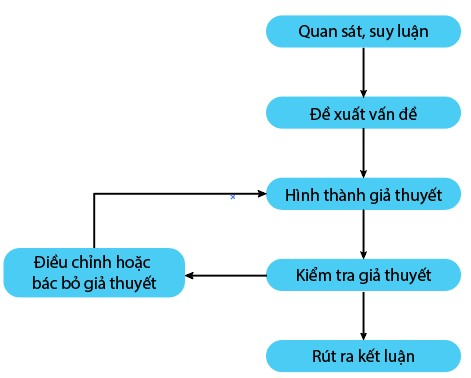
\includegraphics[scale=0.7]{figs/G10Y25B1-2}
	\end{center}
	\subsubsection{Quá trình phát triển của vật lí}
	\begin{center}
		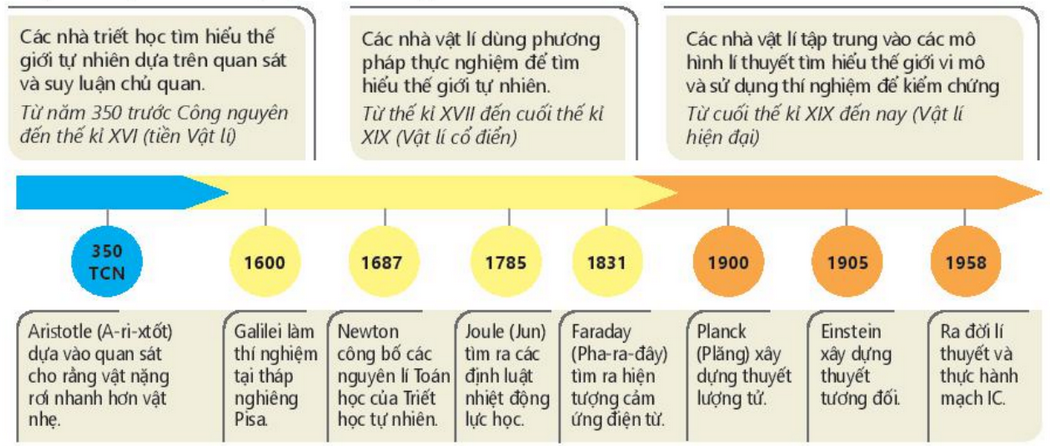
\includegraphics[scale=0.9]{figs/G10Y25B1-1}
	\end{center}
	\subsubsection{Vai trò của vật lí đối với khoa học, kĩ thuật và công nghệ}
	\paragraph{Thông tin liên lạc}
	Khoảng cách địa lí không còn là vấn đề quá lớn của con người trong thông tin liên lạc, sự bùng nổ của mạng lưới internet kết hợp sự phát triển vượt bậc của điện thoại thông minh (smartphone) giúp con người có thể chia sẻ thông tin liên lạc (hình ảnh, giọng nói, tin tức...) một cách dễ dàng.
	\paragraph{Y tế}
	Hầu hết các phương pháp chuẩn đoán và chữa bệnh trong y học đều có cơ sở từ những kiến thức Vật Lý như: chụp X – quang, chụp cộng hưởng từ (MRI), siêu âm, nội soi, xạ trị, \dots
	\paragraph{Công nghiệp}
	Cuộc cách mạng công nghiệp lần thứ tư được coi là bắt đầu thế kỉ XXI. Các nền sản xuất thủ công nhỏ lẻ được thay thế bởi những dây chuyền sản xuất tự động hóa, sử dụng trí tuệ nhân tạo, công nghệ vật liệu (nano), điện toán đám mây.
	\paragraph{Nông nghiệp}
	Việc ứng dụng những thành tựu của Vật Lý vào nông nghiệp đã giúp cho người nông dân tiếp cận với nhiều phương pháp mới, ít tốn lao động, cho năng suất cao. 
	\paragraph{Nghiên cứu khoa học}
	Vật lý góp phần to lớn trong việc cải tiến các thiết bị nghiên cứu khoa học ở nhiều ngành khác nhau như: kính hiển vi điện tử, nhiễu xạ tia X, máy quang phổ, \dots
\end{tomtat}
\subsubsection{Vấn đề an toàn trong Vật lí}
\paragraph{An toàn khi làm việc với phóng xạ}
\begin{enumerate}[label=\arabic*)]
	\item Giữ khoảng cách đủ xa đối với nguồn phóng xạ.
	\item Sử dụng các tấm chắn nguồn phóng xạ đủ tốt.
	\item Giảm thiểu thời gian phơi nhiễm phóng xạ.
\end{enumerate}
\begin{center}
	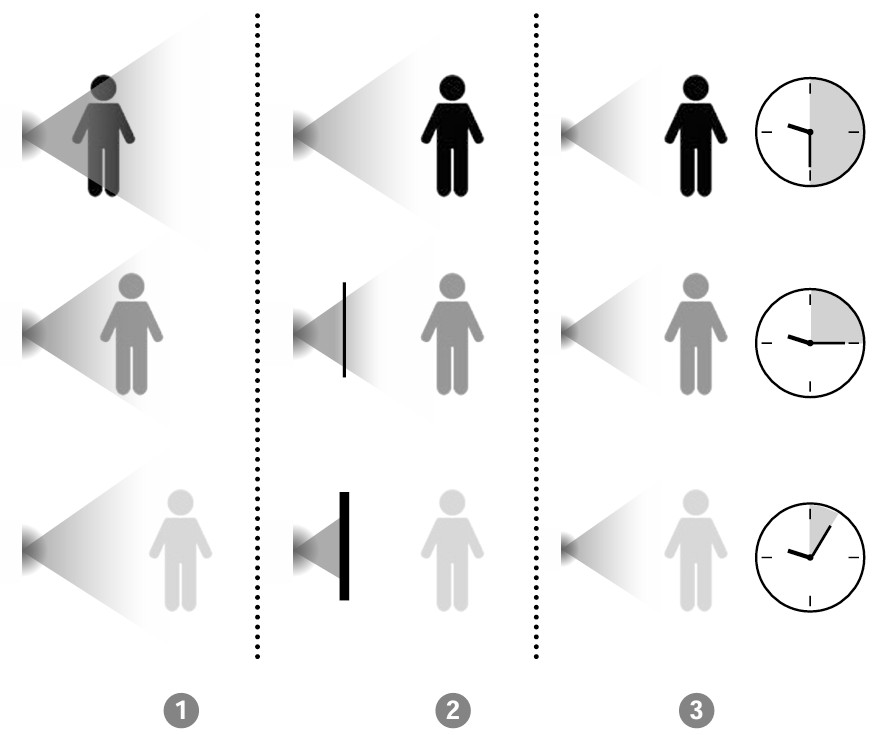
\includegraphics[scale=0.6]{figs/G10Y25B1-3}
\end{center}
\subsubsection{An toàn trong phòng thí nghiệm}
\begin{enumerate}[label=\alph*)]
	\item Một số biện pháp an toàn khi sử dụng điện:
	\begin{itemize}
		\item Trang bị đầy đủ các thiết bị bảo hộ cá nhân.
		\item Giữ khoảng cách an toàn với nguồn điện.
		\item Tránh sử dụng các thiết bị điện khi đang sạc.
		\item Không dùng tay ướt hoặc nhiều mồ hôi khi sử dụng dây điện.
		\item Tránh xa nơi điện thế nguy hiểm.
		\item Lắp đặt vị trí cầu dao, cầu chì, công tắc, ổ điện đúng quy định, \dots
	\end{itemize}
	\item  Khi nghiên cứu và học tập Vật lí cần phải:
	\begin{itemize}
		\item Hiểu được thông tin liên quan đến các rủi ro và nguy hiểm có thể xảy ra.
		\item Tuân thủ và áp dụng các biện pháp bảo vệ để đảm bảo an toàn cho bản thân và cộng đồng.
		\item Quan tâm, gìn giữ và bảo vệ môi trường.
		\item Trong phòng thí nghiệm ở trường học, những rủi ro và nguy hiểm phải được cảnh báo rõ ràng bằng các biển báo. Học sinh cần chú ý sự nhắc nhở của nhân viên phòng thí nghiệm và giáo viên về các quy định an toàn. Ngoài ra, các thiết bị bảo hộ cá nhân cần phải được trang bị đầy đủ.
	\end{itemize}
\end{enumerate}
\subsection{VÍ DỤ MINH HỌA}
\begin{dang}{Phân tích phương trình chuyển động}
	$$x=x_0+vt.$$
	\end{dang}
	% ===================================================================
	\begin{vd}
		
		\choice
		{}
		{}
		{}
		{}
		\loigiai{}
	\end{vd}
\begin{dang}{Nêu được ví dụ về các phương pháp nghiên cứu vật lí}
\end{dang}
\begin{vd}
	Vào đầu thế kỉ XX, J.J.Thomson đã đề xuất mô hình cấu tạo nguyên tử gồm các electron phân bố đều trong một khối điện dương kết cấu tựa như khối mây. Để kiểm chứng giả thuyết này, E. Rutherford đã sử dụng tia alpha gồm các hạt mang điện dương bắn vào các nguyên tử kim loại vàng Hình \ref{fig:2.2}. Kết quả của thí nghiệm đã bác bỏ giả thuyết của J. J. Thomson, đồng thời đã giúp khám phá ra hạt nhân nguyên tử. E. Rutherford đã vận dụng phương pháp nghiên cứu nào để nghiên cứu vấn đề này? Giải thích.
	\begin{center}
		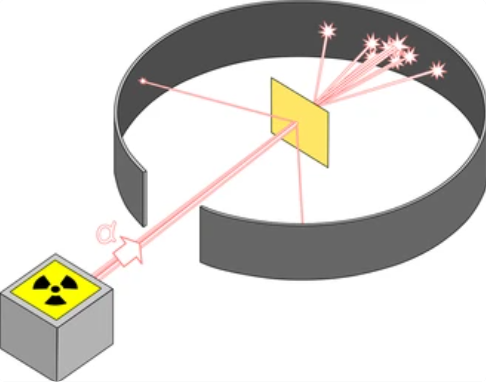
\includegraphics[scale=0.3]{figs/G10Y25B1-4}
		\captionof{figure}{Thí nghiệm Rutherford.}
		\label{fig:2.2}
	\end{center}
	\loigiai{
		Rutherford đã sử dụng phương pháp thực nghiệm trong nghiên cứu vật lí vì ông đã thực hiện thí nghiệm dùng tia alpha gồm các hạt mang điện dương bắn vào các nguyên tử vàng để phát hiện ra kết quả mới chính là hạt nhân nguyên tử.
	}
\end{vd}
\begin{dang}{Mô tả được các bước \\trong tiến trình tìm hiểu thế giới tự nhiên}
\end{dang}
\begin{vd}
	Sắp xếp các bước tiến hành quá trình tìm hiểu thế giới tự nhiên dưới góc độ vật lí:
	\begin{enumerate}[label= (\arabic*)]
		\item Phân tích số liệu.
		\item Quan sát, xác định đối tượng cần nghiên cứu.
		\item Thiết kế, xây dựng mô hình kiểm chứng giả thuyết.
		\item Đề xuất giả thuyết nghiên cứu.
		\item Rút ra kết luận.
	\end{enumerate}
	\loigiai{
		Tiến trình tìm hiểu thế giới tự nhiên dưới góc độ Vật lí là (2) - (4) - (3) - (1) - (5).
	}
\end{vd}
\subsection{TRẮC NGHIỆM NHIỀU PHƯƠNG ÁN LỰA CHỌN}
\setcounter{ex}{0}
\Opensolutionfile{ans}[ans/G10Y25B1-TN]
\begin{ex}
	Đối tượng nghiên cứu của Vật lí là gì?
	\choice
	{Các dạng vận động và tương tác của vật chất}
	{Quy luật tương tác của các dạng năng lượng}
	{\True Các dạng vận động của vật chất và năng lượng}
	{Quy luật vận động, phát triển của sự vật - hiện tượng}
	\loigiai{}
\end{ex}

\begin{ex}
	Lĩnh vực nghiên cứu nào sau đây là của Vật lí?
	\choice
	{Nghiên cứu về sự thay đổi của các chất khi kết hợp với nhau}
	{Nghiên cứu sự phát triển của vi khuẩn}
	{Nghiên cứu về sự hình thành và phát triển của các tầng lớp, giai cấp trong xã hội}
	{\True Nghiên cứu về các dạng chuyển động và các dạng năng lượng khác nhau}
	\loigiai{}
\end{ex}

\begin{ex}
	Cách sắp xếp nào sau đây trong 5 bước của phương pháp thực nghiệm là đúng?
	\choice
	{Xác định vấn đề cần nghiên cứu, dự đoán, quan sát, thí nghiệm, kết luận}
	{Quan sát, xác định vấn đề cần nghiên cứu, thí nghiệm, dự đoán, kết luận}
	{\True Xác định vấn đề cần nghiên cứu, quan sát, dự đoán, thí nghiệm, kết luận}
	{Thí nghiệm, xác định vấn đề cần nghiên cứu, dự đoán, quan sát, kết luận}
	\loigiai{}
\end{ex}

\begin{ex}
	Thành tựu nghiên cứu nào sau đây của Vật lí được coi là có vai trò quan trọng trong việc mở đầu cho cuộc cách mạng công nghệ lần thứ nhất?
	\choice
	{Nghiên cứu về lực vạn vật hấp dẫn}
	{\True Nghiên cứu về nhiệt động lực học}
	{Nghiên cứu về cảm ứng điện từ}
	{Nghiên cứu về thuyết tương đối}
	\loigiai{}
\end{ex}
\begin{ex}
	Trong các hoạt động dưới đây, những hoạt động nào tuân thủ nguyên tắc an toàn khi sử dụng điện?
	\choice
	{Bọc kĩ các dây dẫn điện bằng vật liệu cách điện}
	{Kiểm tra mạch có điện bằng bút thử điện}
	{Sửa chữa điện khi chưa ngắt nguồn điện}
	{Chạm tay trực tiếp vào ổ điện, dây điện trần hoặc dây dẫn điện bị hở}
	{Thường xuyên kiểm tra tình trạng hệ thống đường điện và các đồ dùng điện}
	{Đến gần nhưng không tiếp xúc với các máy biến thế và lưới điện cao áp}
	\loigiai{\textbf{Đáp án: A, B, E.}}
\end{ex}

\begin{ex}
	Trong các hoạt động dưới đây, những hoạt động nào tuân thủ nguyên tắc an toàn khi làm việc với các nguồn phóng xạ?
	\choice
	{Sử dụng phương tiện phòng hộ cá nhân như quần áo phòng hộ, mũ, găng tay, áo chì, \dots}
	{Ăn uống, trang điểm trong phòng làm việc có chứa chất phóng xạ}
	{Tẩy xạ khi bị nhiễm bẩn phóng xạ theo quy định}
	{Đổ rác thải phóng xạ tại các khu tập trung rác thải sinh hoạt}
	{Kiểm tra sức khoẻ định kì}
	\loigiai{\textbf{Đáp án: A, C, E.}}
\end{ex}
\Closesolutionfile{ans}
\subsection{TRẮC NGHIỆM ĐÚNG SAI}
\setcounter{ex}{0}
\Opensolutionfile{ans}[ans/G10Y25B1-TF]
% ===================================================================
\begin{ex}
	
	\choiceTF[t]
	{}
	{}
	{}
	{}
	\loigiai{}
\end{ex}
\Closesolutionfile{ans}
\subsection{TỰ LUẬN}
\setcounter{ex}{0}
\Opensolutionfile{ans}[ans/G10Y25B1-TL]

\Closesolutionfile{ans}